\hypertarget{widgets-3}{%
\section{Widgets (3)}\label{widgets-3}}

\hypertarget{open-signal}{%
\subsection{Open signal}\label{open-signal}}

\hypertarget{g_application_handles_open-flag}{%
\subsubsection{G\_APPLICATION\_HANDLES\_OPEN
flag}\label{g_application_handles_open-flag}}

The GtkTextView, GtkTextBuffer and GtkScrolledWindow widgets have given
us a minimum editor in the previous section. We will now add a function
to read a file and rework the program into a file viewer. There are many
ways to implement the function and because this is a tutorial for
beginners, we'll take the easiest one.

When the program starts, we will give the filename to open as an
argument.

\begin{lstlisting}
$ ./a.out filename
\end{lstlisting}

It will open the file and insert its contents into the GtkTextBuffer.

To do this, we need to know how GtkApplication (or GApplication)
recognizes arguments. This is described in the
\href{https://docs.gtk.org/gio/class.Application.html}{GIO API
Reference, Application}.

When GtkApplication is created, a flag (with the type GApplicationFlags)
is provided as an argument.

\begin{lstlisting}[language=C]
GtkApplication *
gtk_application_new (const gchar *application_id, GApplicationFlags flags);
\end{lstlisting}

This tutorial explains only two flags,
\passthrough{\lstinline!G\_APPLICATION\_FLAGS\_NONE!} and
\passthrough{\lstinline!G\_APPLICATION\_HANDLES\_OPEN!}. If you want to
handle command line arguments, the
\passthrough{\lstinline!G\_APPLICATION\_HANDLES\_COMMAND\_LINE!} flag is
what you need. How to use the new application method is described in
\href{https://docs.gtk.org/gio/method.Application.run.html}{GIO API
Reference, g\_application\_run}, and the flag is described in the
\href{https://docs.gtk.org/gio/flags.ApplicationFlags.html}{GIO API
Reference, ApplicationFlags}.

\begin{lstlisting}
GApplicationFlags' Members

G_APPLICATION_FLAGS_NONE  Default. (No argument allowed)
  ... ... ...
G_APPLICATION_HANDLES_OPEN  This application handles opening files (in the primary instance).
  ... ... ...
\end{lstlisting}

There are ten flags in total, but we only need two of them so far. We've
already used \passthrough{\lstinline!G\_APPLICATION\_FLAGS\_NONE!}, as
it is the simplest option, and no arguments are allowed. If you provide
arguments when running the application, an error will occur.

The flag \passthrough{\lstinline!G\_APPLICATION\_HANDLES\_OPEN!} is the
second simplest option. It allows arguments but only files. The
application assumes all the arguments are filenames and we will use this
flag when creating our GtkApplication.

\begin{lstlisting}[language=C]
app = gtk_application_new ("com.github.ToshioCP.tfv3", G_APPLICATION_HANDLES_OPEN);
\end{lstlisting}

\hypertarget{open-signal-1}{%
\subsubsection{open signal}\label{open-signal-1}}

Now, when the application starts, two signals can be emitted.

\begin{itemize}
\tightlist
\item
  activate signal --- This signal is emitted when there's no argument.
\item
  open signal --- This signal is emitted when there is at least one
  argument.
\end{itemize}

The handler of the ``open'' signal is defined as follows.

\begin{lstlisting}[language=C]
void user_function (GApplication *application,
                   gpointer      files,
                   gint          n_files,
                   gchar        *hint,
                   gpointer      user_data)
\end{lstlisting}

The parameters are:

\begin{itemize}
\tightlist
\item
  \passthrough{\lstinline!application!} --- the application (usually
  GtkApplication)
\item
  \passthrough{\lstinline!files!} --- an array of GFiles. {[}array
  length=n\_files{]} {[}element-type GFile{]}
\item
  \passthrough{\lstinline!n\_files!} --- the number of the elements of
  \passthrough{\lstinline!files!}
\item
  \passthrough{\lstinline!hint!} --- a hint provided by the calling
  instance (usually it can be ignored)
\item
  \passthrough{\lstinline!user\_data!} --- user data set when the signal
  handler was connected.
\end{itemize}

How to read a specified file (GFile) will be described next.

\hypertarget{making-a-file-viewer}{%
\subsection{Making a file viewer}\label{making-a-file-viewer}}

\hypertarget{what-is-a-file-viewer}{%
\subsubsection{What is a file viewer?}\label{what-is-a-file-viewer}}

A file viewer is a program that displays the text file that is given as
an argument. Our file viewer will work as follows.

\begin{itemize}
\tightlist
\item
  When arguments are given, it treats the first argument as a filename
  and opens it.
\item
  If opening the file succeeds, it reads the contents of the file and
  inserts it to GtkTextBuffer and then shows the window.
\item
  If it fails to open the file, it will show an error message and quit.
\item
  If there's no argument, it will shows an error message and quit.
\item
  If there are two or more arguments, the second one and any others are
  ignored.
\end{itemize}

The program which does this is shown below.

\begin{lstlisting}[language=C, numbers=left]
#include <gtk/gtk.h>

static void
app_activate (GApplication *app, gpointer user_data) {
  g_print ("You need a filename argument.\n");
}

static void
app_open (GApplication *app, GFile ** files, gint n_files, gchar *hint, gpointer user_data) {
  GtkWidget *win;
  GtkWidget *scr;
  GtkWidget *tv;
  GtkTextBuffer *tb;
  char *contents;
  gsize length;
  char *filename;

  win = gtk_application_window_new (GTK_APPLICATION (app));
  gtk_window_set_default_size (GTK_WINDOW (win), 400, 300);

  scr = gtk_scrolled_window_new ();
  gtk_window_set_child (GTK_WINDOW (win), scr);

  tv = gtk_text_view_new ();
  tb = gtk_text_view_get_buffer (GTK_TEXT_VIEW (tv));
  gtk_text_view_set_wrap_mode (GTK_TEXT_VIEW (tv), GTK_WRAP_WORD_CHAR);
  gtk_text_view_set_editable (GTK_TEXT_VIEW (tv), FALSE);
  gtk_scrolled_window_set_child (GTK_SCROLLED_WINDOW (scr), tv);

  if (g_file_load_contents (files[0], NULL, &contents, &length, NULL, NULL)) {
    gtk_text_buffer_set_text (tb, contents, length);
    g_free (contents);
    if ((filename = g_file_get_basename (files[0])) != NULL) {
      gtk_window_set_title (GTK_WINDOW (win), filename);
      g_free (filename);
    }
    gtk_widget_show (win);
  } else {
    if ((filename = g_file_get_path (files[0])) != NULL) {
      g_print ("No such file: %s.\n", filename);
      g_free (filename);
    }
    gtk_window_destroy (GTK_WINDOW (win));
  }
}

int
main (int argc, char **argv) {
  GtkApplication *app;
  int stat;

  app = gtk_application_new ("com.github.ToshioCP.tfv3", G_APPLICATION_HANDLES_OPEN);
  g_signal_connect (app, "activate", G_CALLBACK (app_activate), NULL);
  g_signal_connect (app, "open", G_CALLBACK (app_open), NULL);
  stat = g_application_run (G_APPLICATION (app), argc, argv);
  g_object_unref (app);
  return stat;
}
\end{lstlisting}

Save it as \passthrough{\lstinline!tfv3.c!}. Then compile and run it.

\begin{lstlisting}
$ comp tfv3
$ ./a.out tfv3.c
\end{lstlisting}

\begin{figure}
\centering
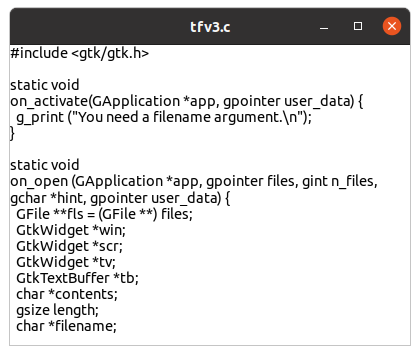
\includegraphics[width=6.3cm,height=5.325cm]{../image/screenshot_tfv3.png}
\caption{File viewer}
\end{figure}

Let's explain how the program \passthrough{\lstinline!tfv3.c!} works.
First, the function \passthrough{\lstinline!main!} has only two changes
from the previous version.

\begin{itemize}
\tightlist
\item
  \passthrough{\lstinline!G\_APPLICATION\_FLAGS\_NONE!} is replaced by
  \passthrough{\lstinline!G\_APPLICATION\_HANDLES\_OPEN!}; and
\item
  \passthrough{\lstinline!g\_signal\_connect (app, "open", G\_CALLBACK (on\_open), NULL)!}
  is added.
\end{itemize}

Next, the handler \passthrough{\lstinline!app\_activate!} is added and
is very simple. It just outputs the error message and the application
quits immediately because no window is created.

The main functionality is the in the handler
\passthrough{\lstinline!app\_open!}. It

\begin{itemize}
\tightlist
\item
  Creates GtkApplicationWindow, GtkScrolledWindow, GtkTextView and
  GtkTextBuffer and connects them together;
\item
  Sets wrap mode to \passthrough{\lstinline!GTK\_WRAP\_WORD\_CHAR!} in
  GtktextView;
\item
  Sets GtkTextView to non-editable because the program isn't an editor
  but only a viewer;
\item
  Reads the file and inserts the text into GtkTextBuffer (this will be
  explained in detail later); and
\item
  If the file is not opened then outputs an error message and destroys
  the window. This makes the application quit.
\end{itemize}

The following is the important file reading part of the program and is
shown again below.

\begin{lstlisting}[language=C]
if (g_file_load_contents (files[0], NULL, &contents, &length, NULL, NULL)) {
  gtk_text_buffer_set_text (tb, contents, length);
  g_free (contents);
  if ((filename = g_file_get_basename (files[0])) != NULL) {
    gtk_window_set_title (GTK_WINDOW (win), filename);
    g_free (filename);
  }
  gtk_widget_show (win);
} else {
  if ((filename = g_file_get_path (files[0])) != NULL) {
    g_print ("No such file: %s.\n", filename);
    g_free (filename);
  }
  gtk_window_destroy (GTK_WINDOW (win));
}
\end{lstlisting}

The function \passthrough{\lstinline!g\_file\_load\_contents!} loads the
file contents into a buffer, which is automatically allocated and sets
\passthrough{\lstinline!contents!} to point that buffer. The length of
the buffer is set to \passthrough{\lstinline!length!}. It returns
\passthrough{\lstinline!TRUE!} if the file's contents are successfully
loaded and \passthrough{\lstinline!FALSE!} if an error occurs.

If this function succeeds, it inserts the contents into GtkTextBuffer,
frees the buffer pointed by \passthrough{\lstinline!contents!}, sets the
title of the window, frees the memories pointed by
\passthrough{\lstinline!filename!} and then shows the window. If it
fails, it outputs an error message and destroys the window, causing the
program to quit.

\hypertarget{gtknotebook}{%
\subsection{GtkNotebook}\label{gtknotebook}}

GtkNotebook is a container widget that uses tabs and contains multiple
children. The child that is displayed depends on which tab has been
selected.

\begin{figure}
\centering
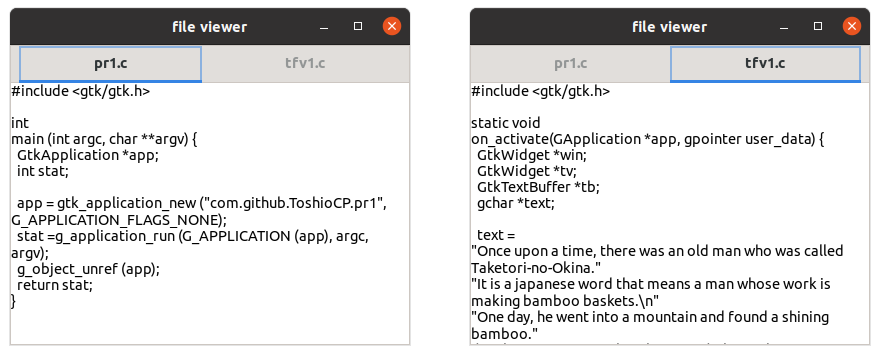
\includegraphics[width=13.2cm,height=5.325cm]{../image/screenshot_gtk_notebook.png}
\caption{GtkNotebook}
\end{figure}

Looking at the screenshots above, the left one is the window at the
startup. It shows the file \passthrough{\lstinline!pr1.c!} and the
filename is in the left tab. After clicking on the right tab, the
contents of the file \passthrough{\lstinline!tfv1.c!} are shown instead.
This is shown in the right screenshot.

The GtkNotebook widget is inserted as a child of GtkApplicationWindow
and contains a GtkScrolledWindow for each file that is being displayed.
The code to do this is given in \passthrough{\lstinline!tfv4.c!} and is:

\begin{lstlisting}[language=C, numbers=left]
#include <gtk/gtk.h>

static void
app_activate (GApplication *app, gpointer user_data) {
  g_print ("You need a filename argument.\n");
}

static void
app_open (GApplication *app, GFile ** files, gint n_files, gchar *hint, gpointer user_data) {
  GtkWidget *win;
  GtkWidget *nb;
  GtkWidget *lab;
  GtkNotebookPage *nbp;
  GtkWidget *scr;
  GtkWidget *tv;
  GtkTextBuffer *tb;
  char *contents;
  gsize length;
  char *filename;
  int i;

  win = gtk_application_window_new (GTK_APPLICATION (app));
  gtk_window_set_title (GTK_WINDOW (win), "file viewer");
  gtk_window_set_default_size (GTK_WINDOW (win), 400, 300);
  gtk_window_maximize (GTK_WINDOW (win));

  nb = gtk_notebook_new ();
  gtk_window_set_child (GTK_WINDOW (win), nb);

  for (i = 0; i < n_files; i++) {
    if (g_file_load_contents (files[i], NULL, &contents, &length, NULL, NULL)) {
      scr = gtk_scrolled_window_new ();
      tv = gtk_text_view_new ();
      tb = gtk_text_view_get_buffer (GTK_TEXT_VIEW (tv));
      gtk_text_view_set_wrap_mode (GTK_TEXT_VIEW (tv), GTK_WRAP_WORD_CHAR);
      gtk_text_view_set_editable (GTK_TEXT_VIEW (tv), FALSE);
      gtk_scrolled_window_set_child (GTK_SCROLLED_WINDOW (scr), tv);

      gtk_text_buffer_set_text (tb, contents, length);
      g_free (contents);
      if ((filename = g_file_get_basename (files[i])) != NULL) {
        lab = gtk_label_new (filename);
        g_free (filename);
      } else
        lab = gtk_label_new ("");
      gtk_notebook_append_page (GTK_NOTEBOOK (nb), scr, lab);
      nbp = gtk_notebook_get_page (GTK_NOTEBOOK (nb), scr);
      g_object_set (nbp, "tab-expand", TRUE, NULL);
    } else if ((filename = g_file_get_path (files[i])) != NULL) {
        g_print ("No such file: %s.\n", filename);
        g_free (filename);
    } else
        g_print ("No valid file is given\n");
  }
  if (gtk_notebook_get_n_pages (GTK_NOTEBOOK (nb)) > 0)
    gtk_widget_show (win);
  else
    gtk_window_destroy (GTK_WINDOW (win));
}

int
main (int argc, char **argv) {
  GtkApplication *app;
  int stat;

  app = gtk_application_new ("com.github.ToshioCP.tfv4", G_APPLICATION_HANDLES_OPEN);
  g_signal_connect (app, "activate", G_CALLBACK (app_activate), NULL);
  g_signal_connect (app, "open", G_CALLBACK (app_open), NULL);
  stat = g_application_run (G_APPLICATION (app), argc, argv);
  g_object_unref (app);
  return stat;
}
\end{lstlisting}

Most of the changes are in the function
\passthrough{\lstinline!app\_open!}. The numbers at the left of the
following items are line numbers in the source code.

\begin{itemize}
\tightlist
\item
  11-13: Variables \passthrough{\lstinline!nb!},
  \passthrough{\lstinline!lab!} and \passthrough{\lstinline!nbp!} are
  defined and will point to a new GtkNotebook, GtkLabel and
  GtkNotebookPage widget respectively.
\item
  23: The window's title is set to ``file viewer''.
\item
  25: The size of the window is set to maximum because a big window is
  appropriate for file viewers.
\item
  27-28 GtkNotebook is created and inserted to the GtkApplicationWindow
  as a child.
\item
  30-59 For-loop. Each loop corresponds to a filename argument, and
  \passthrough{\lstinline!files[i]!} is GFile object containing the i-th
  argument.
\item
  32-37 GtkScrollledWindow, GtkTextView are created and GtkTextBuffer
  found from the new GtkTextView. GtkTextView is connected to
  GtkScrolledWindow as a child. Each file gets their own copy of these
  widgets, so they are created inside the for-loop.
\item
  39-40 inserts the contents of the file into GtkTextBuffer and frees
  the memory pointed by \passthrough{\lstinline!contents!}.
\item
  41-43: Gets the filename and creates GtkLabel with the filename and
  then frees \passthrough{\lstinline!filename!}.
\item
  44-45: If \passthrough{\lstinline!filename!} is NULL, creates GtkLabel
  with the empty string.
\item
  46: Appends GtkScrolledWindow as a page, with the tab GtkLabel, to
  GtkNotebook. At this time a GtkNoteBookPage widget is created
  automatically. The GtkScrolledWindow widget is connected to the
  GtkNotebookPage. Therefore, the structure is like this:
\end{itemize}

\begin{lstlisting}
    GtkNotebook -- GtkNotebookPage -- GtkScrolledWindow
\end{lstlisting}

\begin{itemize}
\tightlist
\item
  47: Gets GtkNotebookPage widget and sets \passthrough{\lstinline!nbp!}
  to point to this GtkNotebookPage.
\item
  48: GtkNotebookPage has a property set called ``tab-expand''. If it is
  set to TRUE then the tab expands horizontally as long as possible. If
  it is FALSE, then the width of the tab is determined by the size of
  the label. \passthrough{\lstinline!g\_object\_set!} is a general
  function to set properties in objects. See
  \href{https://docs.gtk.org/gobject/method.Object.set.html}{GObject API
  Reference, g\_object\_set}.
\item
  49-51: If the file cannot be read, ``No such file'' message is
  displayed and the \passthrough{\lstinline!filename!} buffer is freed.
\item
  52-53: If \passthrough{\lstinline!filename!} is NULL, the ``No valid
  file is given'' message is outputted.
\item
  55-58: If at least one file was read, then the number of
  GtkNotebookPage is greater than zero. If it's true, it shows the
  window. If it's false, it destroys the window, which causes the
  program to quit.
\end{itemize}
